\documentclass[xcolor=dvipsnames]{beamer}
\usepackage[utf8]{inputenc}
\usepackage{comment}
\usepackage{pgfplots}
\pgfplotsset{compat=newest}
\usetikzlibrary{pgfplots.groupplots}
\usetikzlibrary{shapes,arrows,shadows,shadows.blur,positioning,calc,arrows.meta,automata}
\usetikzlibrary{matrix,calc,decorations.pathreplacing}
\usepackage{pgfpages}
\usetheme{Berlin}
\usecolortheme{default}
\setbeamercolor*{structure}{bg=white,fg=black}
\setbeamertemplate{enumerate items}[default]
\usepackage{times,url}
\makeatletter
\newcommand{\nonumsec}[1]{%
\section*{#1}%
\addtocontents{toc}{\protect\beamer@sectionintoc{\the\c@section}{#1}{\the\c@page}{\the\c@part}%
        {0}}%
}
\makeatother

\setbeamertemplate{headline}
{%
  \begin{beamercolorbox}[colsep=1.5pt]{upper separation line head}
  \end{beamercolorbox}
  \begin{beamercolorbox}{section in head/foot}
    \vskip2pt\insertnavigation{\paperwidth}\vskip2pt
  \end{beamercolorbox}%
  \begin{beamercolorbox}[colsep=1.5pt]{lower separation line head}
  \end{beamercolorbox}
}

\addtobeamertemplate{navigation symbols}{}{%
    \usebeamerfont{footline}%
    \usebeamercolor[fg]{footline}%
    \hspace{1em}%
    \insertframenumber/\inserttotalframenumber
}
%--------------------------------------------------------------------------------------------------
%This block of code defines the information to appear in the
%Title page

\title[] %Learning Discriminative Representations to Interpret Image Recognition Models
{Learning Discriminative Representations to Interpret Image Recognition Models}
\subtitle{Thèse de Doctorat}
\author[Felipe Torres Figueroa] % (optional)
{Felipe Torres Figueroa}
\institute[ECM] % (optional)
{
  \'Ecole Centrale de Marseille
  \and
  Laboratoire d'Informatique et de Syst\`emes (LIS)
}
\date[2024] % (optional)
{Marseille, September 2024}
\logo{%
  \makebox[0.95\paperwidth]{%
    
\includegraphics[height=1cm,keepaspectratio]{logo/logo-lis-2024-eps-converted-to.pdf}%    
    \hfill%
    
\includegraphics[height=1cm,keepaspectratio]{logo/ecm_logo.png}%
  }%
}
%End of title page configuration block
%--------------------------------------------------------------------------------------------------
%The next block of commands puts the table of contents at the 
%beginning of each section and highlights the current section:
\AtBeginSection
{
  \begin{frame}
    \frametitle{Table of Contents}
    \tableofcontents[currentsection]
  \end{frame}
}
%------------------------------------------------------------------------------
% hack for CVPR/ICCV style
\makeatletter
\@namedef{ver@everyshi.sty}{}
\makeatother

%------------------------------------------------------------------------------
% main packages
%\usepackage[dvipsnames,svgnames,x11names]{xcolor}
\usepackage{tikz}
\usetikzlibrary{arrows.meta,shapes,calc,matrix,fit,positioning,backgrounds,decorations.markings,fadings}
\usepackage{pgfplots}
\usepackage{pgfplotstable}
\usepgfplotslibrary{dateplot}
\pgfplotsset{compat=1.9}
\usepackage{xstring}

%------------------------------------------------------------------------------
% externalization: requires defining \finalcopy first

\usepgfplotslibrary{external}
% \tikzexternalize[prefix=fig/extern/]
\newcommand{\extfig}[2]{\tikzsetnextfilename{#1}{#2}}
\newcommand{\noextfig}[1]{\tikzset{external/export next={false}}{#1}}
\newcommand{\extdata}[1]{\input{#1}}
\IfBeginWith*{\jobname}{fig/extern/}{\finalcopy}{}

%-----------------------------------------------------------------------------
% tikz styles

\tikzstyle{every picture}+=[
	remember picture,
	every text node part/.style={align=center},
	every matrix/.append style={ampersand replacement=\&},
]
\tikzstyle{tight} = [inner sep=0pt,outer sep=0pt]
\tikzstyle{node}  = [draw,circle,tight,minimum size=12pt,anchor=center]
\tikzstyle{op}    = [draw,circle,tight]
\tikzstyle{dot}   = [fill,draw,circle,inner sep=1pt,outer sep=0]
\tikzstyle{pt}    = [fill,draw,circle,inner sep=1.5pt,outer sep=.2pt]
\tikzstyle{box}   = [draw,rectangle,inner sep=3pt]
\tikzstyle{high}  = [black!60]
\tikzstyle{group} = [high,box,opacity=.5]
\tikzstyle{dim1}  = [fill opacity=.3,text opacity=1]
\tikzstyle{dim2}  = [fill opacity=.5,text opacity=1]
\tikzstyle{dim3}  = [fill opacity=.7,text opacity=1]
\tikzstyle{rectc} = [tight,transform shape]
\tikzstyle{rect}  = [rectc,anchor=south west]

%-----------------------------------------------------------------------------
% framed figures

\newcommand{\framed}[3][1]{\extfig{#2}{\tikz{
	\node[tight](a){\fig[#1]{#3}};
	\node[tight,draw=gray,fit=(a)]{};
}}}

%-----------------------------------------------------------------------------
% pgfplots general options

\newcommand{\leg}[1]{\addlegendentry{#1}}

\tikzset{every mark/.append style={solid}}
\pgfplotsset{%smooth,
	grid=both, width=\columnwidth, try min ticks=5,
	every axis/.append style={font=\small},
	every axis plot/.append style={thick,mark=none,mark size=1.8,tension=0.18},
	legend cell align=left, legend style={fill opacity=0.8},
	xticklabel={\pgfmathprintnumber[assume math mode=true]{\tick}},
	yticklabel={\pgfmathprintnumber[assume math mode=true]{\tick}},
	nodes near coords math/.style={
	nodes near coords={\pgfmathprintnumber[assume math mode=true]{\pgfplotspointmeta}},
	},
}

\pgfplotsset{
	dash/.style={mark=o,dashed,opacity=0.6},
	dott/.style={mark=o,dotted,opacity=0.6},
	nolim/.style={enlargelimits=false},
	plain/.style={every axis plot/.append style={},nolim,grid=none},
}
%\pgfplotsset{scaled y ticks = false}
\newcommand{\kilo}[1]{\thisrow{#1}/1000}

%--------------------------------------------------------------------

% layers
\pgfdeclarelayer{bg4}
\pgfdeclarelayer{bg3}
\pgfdeclarelayer{bg2}
\pgfdeclarelayer{bg1}
\pgfdeclarelayer{fg1}
\pgfdeclarelayer{fg2}
\pgfdeclarelayer{fg3}
\pgfdeclarelayer{fg4}
\pgfsetlayers{bg4,bg3,bg2,bg1,main,fg1,fg2,fg3,fg4}

%------------------------------------------------------------------------------
% 3d drawing

\pgfkeys{/tikz/.cd, aspect/.store in=\aspect, aspect=1}
\pgfkeys{/tikz/.cd, depth/.store in=\depth, depth=.5}
\pgfkeys{/tikz/.cd, stepx/.store in=\step, stepx=1}

\tikzstyle{geom} = [line join=bevel,aspect=1,depth=.5,z={(\depth*\aspect,\depth)}]
\tikzstyle{wire} = [geom,draw,thick]

% 3d coordinates
\def\cx[#1,#2,#3]{#1}
\def\cy[#1,#2,#3]{#2}
\def\cz[#1,#2,#3]{#3}
\def\ex[#1,#2,#3]{#1,0,0}
\def\ey[#1,#2,#3]{0,#2,0}
\def\ez[#1,#2,#3]{0,0,#3}

% lines along x, y, or z
\newcommand{\zline}[3][]{%
\path[geom,#1] #2 -- +(\cx[#3],\cy[#3]);
}
\newcommand{\yline}[3][]{%
\path[geom,#1,shift={#2},xslant=\aspect]
	(0,0) -- +(\cx[#3],\depth*\cz[#3]);
}
\newcommand{\xline}[3][]{%
\path[geom,#1,shift={#2},yslant=1/\aspect]
	(0,0) -- +(\aspect*\depth*\cz[#3],\cy[#3]);
}

% rectangles / grids along x, y, or z
\newcommand{\zrect}[3][]{%
\path[geom,#1] #2 rectangle +(\cx[#3],\cy[#3]);
}
\newcommand{\yrect}[3][]{%
\path[geom,#1,shift={#2},xslant=\aspect]
	(0,0) rectangle +(\cx[#3],\depth*\cz[#3]);
}
\newcommand{\xrect}[3][]{%
\path[geom,#1,shift={#2},yslant=1/\aspect]
	(0,0) rectangle +(\aspect*\depth*\cz[#3],\cy[#3]);
}
\newcommand{\xgrid}[3][]{%
\path[geom,#1,shift={#2},yslant=1/\aspect,xstep=\aspect*\depth*\step]
	(0,0) grid +(\aspect*\depth*\cz[#3],\cy[#3]);
}

% parallepiped
\newcommand{\para}[4][]{%
\zrect[#1]{(#3)}{#4}                 % front
\yrect[#1]{($(#3)+(\ey[#4])$)}{#4}   % top
\xrect[#1]{($(#3)+(\ex[#4])$)}{#4}   % right
\path[geom]
	(#3) coordinate(#2-southwest)
	($(#3)+(#4)$) coordinate(#2-northeast)
	($(#3)+(\ey[#4])$) coordinate(#2-northwest)
	($(#3)+(#4)-(\ey[#4])$) coordinate(#2-southeast)
	($(#3)+.5*(\ex[#4])$) coordinate(#2-south)
	($(#3)+(#4)-.5*(\ex[#4])$) coordinate(#2-north)
	($(#3)+.5*(\ex[#4])+.5*(#4)$) coordinate(#2-center)
	(#2-southwest |- #2-center) coordinate(#2-west)
	(#2-center -| #2-northeast) coordinate(#2-east)
	;
}


\newcommand{\head}[1]{{\smallskip\noindent\textbf{#1}}}

\newcommand{\sm}{\scriptsize}
\newcommand{\eq}[1]{(\ref{eq:#1})}

\newcommand{\Th}[1]{\textsc{#1}}
\newcommand{\mr}[2]{\multirow{#1}{*}{#2}}
\newcommand{\mc}[2]{\multicolumn{#1}{c}{#2}}
\newcommand{\tb}[1]{\textbf{#1}}
\newcommand{\ch}{\checkmark}

\newcommand{\red}[1]{{\textcolor{red}{#1}}}
\newcommand{\blue}[1]{{\textcolor{blue}{#1}}}
\newcommand{\green}[1]{{\textcolor{green}{#1}}}
%\newcommand{\gray}[1]{{\textcolor{gray}{#1}}}

\newcommand{\citeme}[1]{\red{[XX]}}
\newcommand{\refme}[1]{\red{(XX)}}

\newcommand{\fig}[2][1]{\includegraphics[width=#1\linewidth]{fig/#2}}
\newcommand{\figh}[2][1]{\includegraphics[height=#1\linewidth]{fig/#2}}
\newcommand{\figa}[2][1]{\includegraphics[width=#1]{fig/#2}}
\newcommand{\figah}[2][1]{\includegraphics[height=#1]{fig/#2}}

\newcommand{\tran}{^\top}
\newcommand{\mtran}{^{-\top}}
\newcommand{\zcol}{\mathbf{0}}
\newcommand{\zrow}{\zcol\tran}

\newcommand{\ind}{\mathbbm{1}}
\newcommand{\expect}{\mathbb{E}}
\newcommand{\nat}{\mathbb{N}}
\newcommand{\zahl}{\mathbb{Z}}
%\newcommand{\real}{\mathbb{R}}
\newcommand{\proj}{\mathbb{P}}
\newcommand{\prob}{\operatorname{P}}
\newcommand{\normal}{\mathcal{N}}

\newcommand{\mif}{\textrm{if}\ }
\newcommand{\other}{\textrm{otherwise}}
\newcommand{\minimize}{\textrm{minimize}\ }
\newcommand{\maximize}{\textrm{maximize}\ }
\newcommand{\st}{\textrm{subject\ to}\ }

\newcommand{\id}{\operatorname{id}}
\newcommand{\const}{\operatorname{const}}
\newcommand{\sgn}{\operatorname{sgn}}
%\newcommand{\var}{\operatorname{Var}}
\newcommand{\mean}{\operatorname{mean}}
%\newcommand{\trace}{\operatorname{tr}}
\newcommand{\diag}{\operatorname{diag}}
\newcommand{\vect}{\operatorname{vec}}
\newcommand{\cov}{\operatorname{cov}}
\newcommand{\sign}{\operatorname{sign}}
\newcommand{\prj}{\operatorname{proj}}

\newcommand{\softmax}{\operatorname{softmax}}
\newcommand{\clip}{\operatorname{clip}}

\newcommand{\defn}{\mathrel{:=}}
\newcommand{\peq}{\mathrel{+\!=}}
\newcommand{\meq}{\mathrel{-\!=}}

\newcommand{\paren}[1]{\left({#1}\right)}
\newcommand{\mat}[1]{\left[{#1}\right]}
\newcommand{\set}[1]{\left\{{#1}\right\}}
\newcommand{\floor}[1]{\left\lfloor{#1}\right\rfloor}
\newcommand{\ceil}[1]{\left\lceil{#1}\right\rceil}
\newcommand{\inner}[1]{\left\langle{#1}\right\rangle}
%\newcommand{\norm}[1]{\left\|{#1}\right\|}
%\newcommand{\abs}[1]{\left|{#1}\right|}
%\newcommand{\frob}[1]{\norm{#1}_F}
\newcommand{\card}[1]{\left|{#1}\right|\xspace}

\newcommand{\diff}{\mathrm{d}}
\newcommand{\der}[3][]{\frac{\diff^{#1}#2}{\diff#3^{#1}}}
\newcommand{\ider}[3][]{\diff^{#1}#2/\diff#3^{#1}}
\newcommand{\pder}[3][]{\frac{\partial^{#1}{#2}}{\partial{{#3}^{#1}}}}
\newcommand{\ipder}[3][]{\partial^{#1}{#2}/\partial{#3^{#1}}}
\newcommand{\dder}[3]{\frac{\partial^2{#1}}{\partial{#2}\partial{#3}}}

\newcommand{\wb}[1]{\overline{#1}}
\newcommand{\wt}[1]{\widetilde{#1}}

\def\xssp{\hspace{1pt}}
\def\ssp{\hspace{3pt}}
\def\msp{\hspace{5pt}}
\def\lsp{\hspace{12pt}}

\newcommand{\cA}{\mathcal{A}}
\newcommand{\cB}{\mathcal{B}}
\newcommand{\cC}{\mathcal{C}}
\newcommand{\cD}{\mathcal{D}}
\newcommand{\cE}{\mathcal{E}}
\newcommand{\cF}{\mathcal{F}}
\newcommand{\cG}{\mathcal{G}}
\newcommand{\cH}{\mathcal{H}}
\newcommand{\cI}{\mathcal{I}}
\newcommand{\cJ}{\mathcal{J}}
\newcommand{\cK}{\mathcal{K}}
\newcommand{\cL}{\mathcal{L}}
\newcommand{\cM}{\mathcal{M}}
\newcommand{\cN}{\mathcal{N}}
\newcommand{\cO}{\mathcal{O}}
\newcommand{\cP}{\mathcal{P}}
\newcommand{\cQ}{\mathcal{Q}}
\newcommand{\cR}{\mathcal{R}}
\newcommand{\cS}{\mathcal{S}}
\newcommand{\cT}{\mathcal{T}}
\newcommand{\cU}{\mathcal{U}}
\newcommand{\cV}{\mathcal{V}}
\newcommand{\cW}{\mathcal{W}}
\newcommand{\cX}{\mathcal{X}}
\newcommand{\cY}{\mathcal{Y}}
\newcommand{\cZ}{\mathcal{Z}}

\newcommand{\vA}{\mathbf{A}}
\newcommand{\vB}{\mathbf{B}}
\newcommand{\vC}{\mathbf{C}}
\newcommand{\vD}{\mathbf{D}}
\newcommand{\vE}{\mathbf{E}}
\newcommand{\vF}{\mathbf{F}}
\newcommand{\vG}{\mathbf{G}}
\newcommand{\vH}{\mathbf{H}}
\newcommand{\vI}{\mathbf{I}}
\newcommand{\vJ}{\mathbf{J}}
\newcommand{\vK}{\mathbf{K}}
\newcommand{\vL}{\mathbf{L}}
\newcommand{\vM}{\mathbf{M}}
\newcommand{\vN}{\mathbf{N}}
\newcommand{\vO}{\mathbf{O}}
\newcommand{\vP}{\mathbf{P}}
\newcommand{\vQ}{\mathbf{Q}}
\newcommand{\vR}{\mathbf{R}}
\newcommand{\vS}{\mathbf{S}}
\newcommand{\vT}{\mathbf{T}}
\newcommand{\vU}{\mathbf{U}}
\newcommand{\vV}{\mathbf{V}}
\newcommand{\vW}{\mathbf{W}}
\newcommand{\vX}{\mathbf{X}}
\newcommand{\vY}{\mathbf{Y}}
\newcommand{\vZ}{\mathbf{Z}}

%\newcommand{\va}{\mathbf{a}}
%\newcommand{\vb}{\mathbf{b}}
\newcommand{\vc}{\mathbf{c}}
\newcommand{\vd}{\mathbf{d}}
\newcommand{\ve}{\mathbf{e}}
\newcommand{\vf}{\mathbf{f}}
\newcommand{\vg}{\mathbf{g}}
\newcommand{\vh}{\mathbf{h}}
\newcommand{\vi}{\mathbf{i}}
\newcommand{\vj}{\mathbf{j}}
\newcommand{\vk}{\mathbf{k}}
\newcommand{\vl}{\mathbf{l}}
\newcommand{\vm}{\mathbf{m}}
\newcommand{\vn}{\mathbf{n}}
\newcommand{\vo}{\mathbf{o}}
\newcommand{\vp}{\mathbf{p}}
\newcommand{\vq}{\mathbf{q}}
\newcommand{\vr}{\mathbf{r}}
\newcommand{\Vs}{\mathbf{s}}
\newcommand{\vt}{\mathbf{t}}
\newcommand{\vumod}{\mathbf{u}}
\newcommand{\vv}{\mathbf{v}}
\newcommand{\vw}{\mathbf{w}}
\newcommand{\vx}{\mathbf{x}}
\newcommand{\vy}{\mathbf{y}}
\newcommand{\vz}{\mathbf{z}}

\newcommand{\vone}{\mathbf{1}}
\newcommand{\vzero}{\mathbf{0}}

\newcommand{\valpha}{{\boldsymbol{\alpha}}}
\newcommand{\vbeta}{{\boldsymbol{\beta}}}
\newcommand{\vgamma}{{\boldsymbol{\gamma}}}
\newcommand{\vdelta}{{\boldsymbol{\delta}}}
\newcommand{\vepsilon}{{\boldsymbol{\epsilon}}}
\newcommand{\vzeta}{{\boldsymbol{\zeta}}}
\newcommand{\veta}{{\boldsymbol{\eta}}}
\newcommand{\vtheta}{{\boldsymbol{\theta}}}
\newcommand{\viota}{{\boldsymbol{\iota}}}
\newcommand{\vkappa}{{\boldsymbol{\kappa}}}
\newcommand{\vlambda}{{\boldsymbol{\lambda}}}
\newcommand{\vmu}{{\boldsymbol{\mu}}}
\newcommand{\vnu}{{\boldsymbol{\nu}}}
\newcommand{\vxi}{{\boldsymbol{\xi}}}
\newcommand{\vomikron}{{\boldsymbol{\omikron}}}
\newcommand{\vpi}{{\boldsymbol{\pi}}}
\newcommand{\vrho}{{\boldsymbol{\rho}}}
\newcommand{\vsigma}{{\boldsymbol{\sigma}}}
\newcommand{\vtau}{{\boldsymbol{\tau}}}
\newcommand{\vupsilon}{{\boldsymbol{\upsilon}}}
\newcommand{\vphi}{{\boldsymbol{\phi}}}
\newcommand{\vchi}{{\boldsymbol{\chi}}}
\newcommand{\vpsi}{{\boldsymbol{\psi}}}
\newcommand{\vomega}{{\boldsymbol{\omega}}}


\newcommand{\rLambda}{\mathrm{\Lambda}}
\newcommand{\rSigma}{\mathrm{\Sigma}}

\newcommand{\vLambda}{\bm{\rLambda}}
\newcommand{\vSigma}{\bm{\rSigma}}

\makeatletter
\newcommand*\bdot{\mathpalette\bdot@{.7}}
\newcommand*\bdot@[2]{\mathbin{\vcenter{\hbox{\scalebox{#2}{$\m@th#1\bullet$}}}}}
\makeatother

\makeatletter
\DeclareRobustCommand\onedot{\futurelet\@let@token\@onedot}
\def\@onedot{\ifx\@let@token.\else.\null\fi\xspace}

\def\eg{\emph{e.g}\onedot} \def\Eg{\emph{E.g}\onedot}
\def\ie{\emph{i.e}\onedot} \def\Ie{\emph{I.e}\onedot}
\def\cf{\emph{cf}\onedot} \def\Cf{\emph{Cf}\onedot}
\def\etc{\emph{etc}\onedot} \def\vs{\emph{vs}\onedot}
\def\wrt{w.r.t\onedot} \def\dof{d.o.f\onedot} \def\aka{a.k.a\onedot}
\def\etal{\emph{et al}\onedot}
\makeatother

% ENABLE/DISABLE COMMENTS

% \newcommand{\Col}[2]{{#2}}
% \newcommand{\Note}[2]{}
\newcommand{\Col}[2]{{\color{#1}#2}}
\newcommand{\Note}[2]{[\textbf{#1}: #2]}

\newcommand{\iavr}[1]{\Col{blue}{#1}}
\newcommand{\iavrc}[1]{\iavr{\Note{YA}{#1}}}
\newcommand{\ronan}[1]{\Col{violet}{#1}}
\newcommand{\ronanc}[1]{\ronan{\Note{RS}{#1}}}

% colors

% \definecolor{ForestGreen}{RGB}{34,139,34}
% \definecolor{Orange}{RGB}{1.0, 0.55, 0.0}
% \definecolor{Purple}{RGB}{0.58, 0.44, 0.86}
% \definecolor{LightCyan}{rgb}{0.88,1,1}
% \definecolor{TableColor}{rgb}{0.835, 0.894, 0.968}
\definecolor{darkgreen}{rgb}{0.0, 0.2, 0.13}

% method
\newcommand{\relu}{{\operatorname{ReLU}}}
\newcommand{\gelu}{{\operatorname{GeLU}}}
\newcommand{\conv}{{\operatorname{conv}}}
\newcommand{\avg}{{\operatorname{avg}}}
\newcommand{\fc}{{\textsc{fc}}\xspace}
\newcommand{\gap}{{\textsc{gap}}\xspace}
\newcommand{\mlp}{{\textsc{mlp}}\xspace}
\newcommand{\ca}{{\textsc{ca}}\xspace}
\newcommand{\sa}{{\textsc{sa}}\xspace}
\newcommand{\msa}{{\textsc{msa}}\xspace}
\newcommand{\LN}{{\textsc{ln}}\xspace}
\newcommand{\cls}{{\textsc{cls}}\xspace}
\newcommand{\our}{{\textsc{ca}}}
\newcommand{\ours}{{\textsc{ca}}\xspace}
\newcommand{\Our}{{CA-Stream}}
\newcommand{\Ours}{{CA-Stream}\xspace}
\newcommand{\OURS}{{Cross Attention Stream}\xspace}
\newcommand{\PO}{{\textsc{proj}$\to$\our}\xspace}
\newcommand{\mae}{\textrm{MAE}}
\newcommand{\mse}{\textrm{MSE}}
\newcommand{\hi}{\textrm{HI}}
\definecolor{DarkGreen}{rgb}{0.0, 0.2, 0.13}
%\newcommand{\OM}{{\our$\to$\textsc{mlp}}\xspace}
%\newcommand{\POM}{{\textsc{proj}$\to$\our$\to$\textsc{mlp}}\xspace}
%\newcommand{\we}{\rowcolor{LightCyan}}                       % ours highlighted in table row
%\newcommand{\us}[1]{{\cellcolor{LightCyan}#1}}               % ours highlighted in table cell
\newcommand{\all}{\tikz{\draw[white,fill=black,line width=0.4pt] (0,0) circle (1.2pt);}}

% experiments
\newcommand{\imagenet}{{ImageNet-1k}\xspace}
%\newcommand{\resnet}{{ResNet-$18$}\xspace}
%\newcommand{\resnet50}{{ResNet-$50$}\xspace}
%\newcommand{\vits}{{ViT-S}\xspace}
%\newcommand{\vitt}{{ViT-T}\xspace}
%\newcommand{\convnexts}{{ConvNeXT-S}\xspace}
%\newcommand{\cifar10}{CIFAR-$10$\xspace}
%\newcommand{\cifar100}{CIFAR-$100$\xspace}
%\newcommand{\flowers}{Oxford Flowers\xspace}
%\newcommand{\cub}{CUB-$200$\xspace}
%\newcommand{\voc12}{VOC$12$\xspace}
%\newcommand{\voc7}{VOC$07$\xspace}
%\newcommand{\coco}{COCO\xspace}

\newcommand{\gain}[1]{}
\newcommand{\gp}[1]{{\color{ForestGreen}#1}}
\newcommand{\gn}[1]{\red{#1}}
\newcommand{\se}[1]{\blue{#1}}
\newcommand{\sota}[1]{\red{\textbf{#1}}}
\newcommand{\negative}[1]{\blue{#1}}

\newcommand{\cam}{\textrm{CAM}}
\newcommand{\gcam}{\textrm{Grad-CAM}}
\newcommand{\scam}{\textrm{Score-CAM}}

\newcommand{\Fdef}{Mask\xspace}
\newcommand{\Fref}{Diff\xspace}
\newcommand{\MIOFref}{IODiff\xspace}
\newcommand{\MIODref}{IOMask\xspace}


\newcommand{\AG}{\operatorname{AG}}
\newcommand{\AGf}{Average Gain\xspace}
\newcommand{\Agf}{Average gain\xspace}
\newcommand{\agf}{average gain\xspace}

\newcommand{\AC}{\operatorname{AC}}
\newcommand{\ACf}{Average Contract\xspace}

\newcommand{\AD}{\operatorname{AD}}
\newcommand{\I}{\operatorname{I}}
\newcommand{\D}{\operatorname{D}}
\newcommand{\AI}{\operatorname{AI}}
\newcommand{\OM}{\operatorname{OM}}
\newcommand{\LE}{\operatorname{LE}}
\newcommand{\Fo}{\operatorname{F1}}
\newcommand{\prc}{\operatorname{precision}}
\newcommand{\rec}{\operatorname{recall}}
\newcommand{\BA}{\operatorname{BoxAcc}}
\newcommand{\spg}{\operatorname{SP}}
\newcommand{\epg}{\operatorname{EP}}
\newcommand{\SM}{\operatorname{SM}}
\newcommand{\iou}{\operatorname{IoU}}

\definecolor{TableColor}{rgb}{0.835, 0.894, 0.968}
%--------------------------------------------------------------------------------------------------
\begin{document}
	%The next statement creates the title page.
	{
	\setbeamertemplate{headline}{}
	\begin{frame}
		\maketitle
	\end{frame}
	}
	\logo{}
	%---------------------------------------------------------
	%This block of code is for the table of contents after
	%the title page
	\begin{frame}
		\frametitle{Table of Contents}
		\tableofcontents
	\end{frame}
	\nonumsec{Introduction}	
%--------------------------------------------------------------------------------------------------
\begin{frame}[t]
    \frametitle{Motivation: Low stakes}
    My go to exercise is running, \textbf{but...}\pause
    \begin{figure}
        \centering
        \begin{tikzpicture}[font={\scriptsize}]
            \node[align=center] (text_1) at (0,4) {I think my running shoes \\
                are getting \emph{worn}};
            \node (img_in) at (0, 1.25) {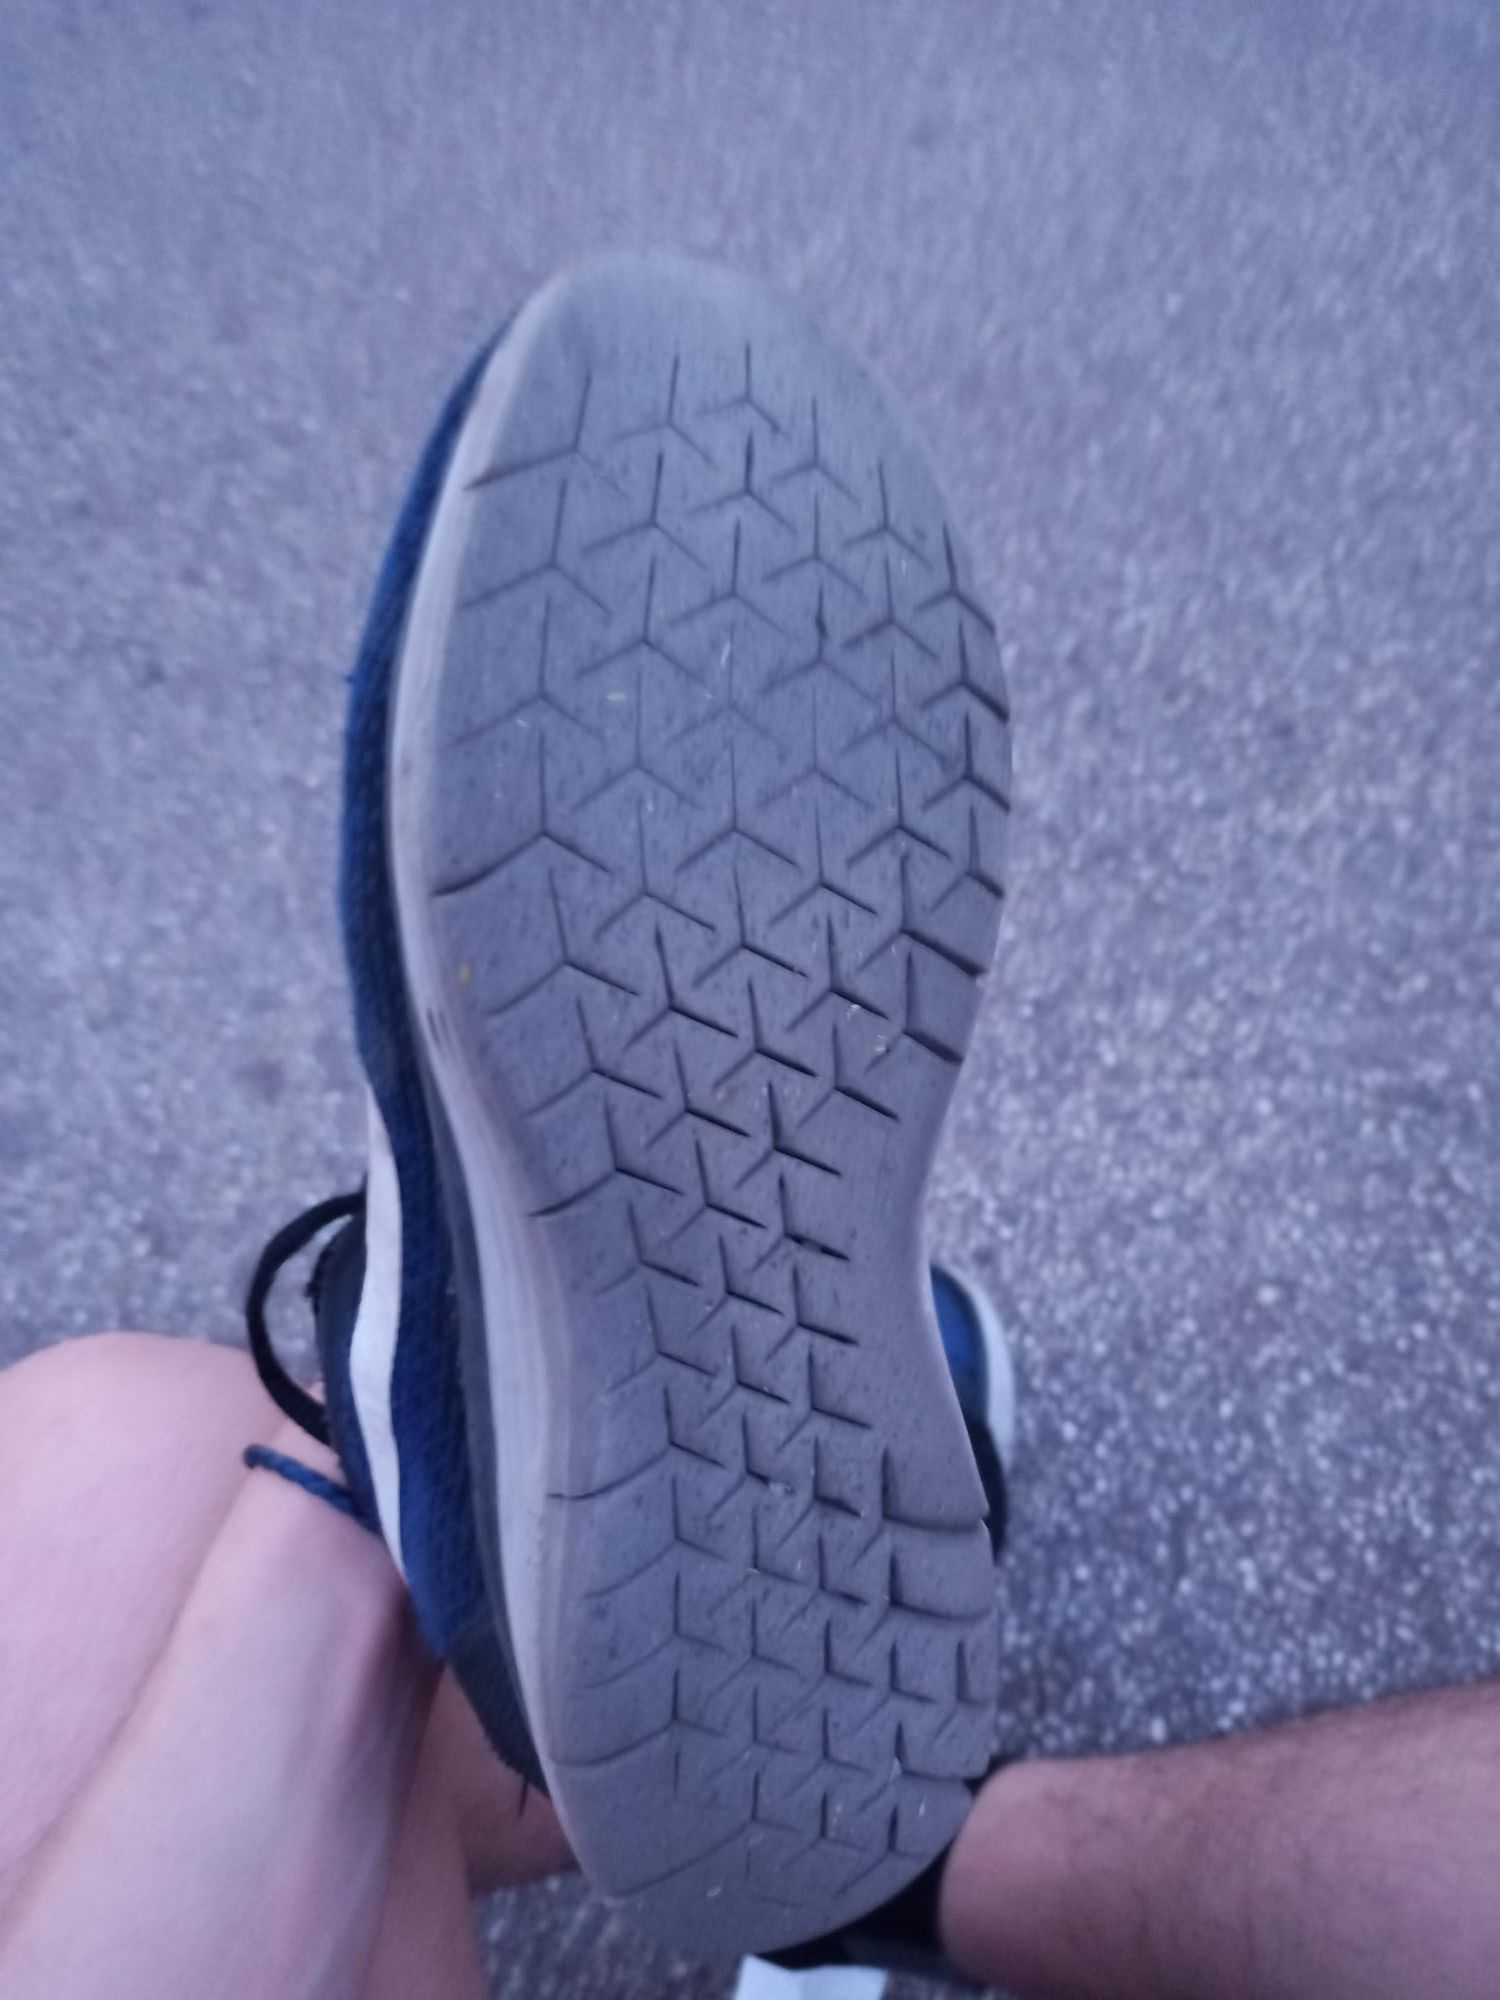
\includegraphics[scale=0.06]
                {fig/intro/motivation/lo_stakes/tired_boss}};
            \pause
            \node[align=center] (text_2) at (3.5, 4) {I want a replacement, \\ 
                 \emph{but} I know about\\machines, not shoes!};
            \pause
            \node[align=center] (text_5) at (3.5, -0.75) {\emph{still}, I know my phone can \\
                \emph{identify} my current shoes};
            \node (img_shoe_raw) at (3.5,1.45) {
\includegraphics[scale=0.07]
                {fig/intro/motivation/lo_stakes/shoe_current}};
            \pause
            \node (img_zeros) at (3.5,1.45) 
                {
\includegraphics[scale=0.1]{fig/intro/motivation/lo_stakes/zeros_img.jpeg}};
            \node (img_idd) at (3.5,1.45) 
                {
\includegraphics[scale=0.09]{fig/intro/motivation/lo_stakes/shoe_lens.jpeg}};
            \node[align=center] (text_brand_new) at (7, 3) {and obtain a new pair \\
                                                of the shoes I like};
            \node (img_brand_new) at (7, 1.75) 
            {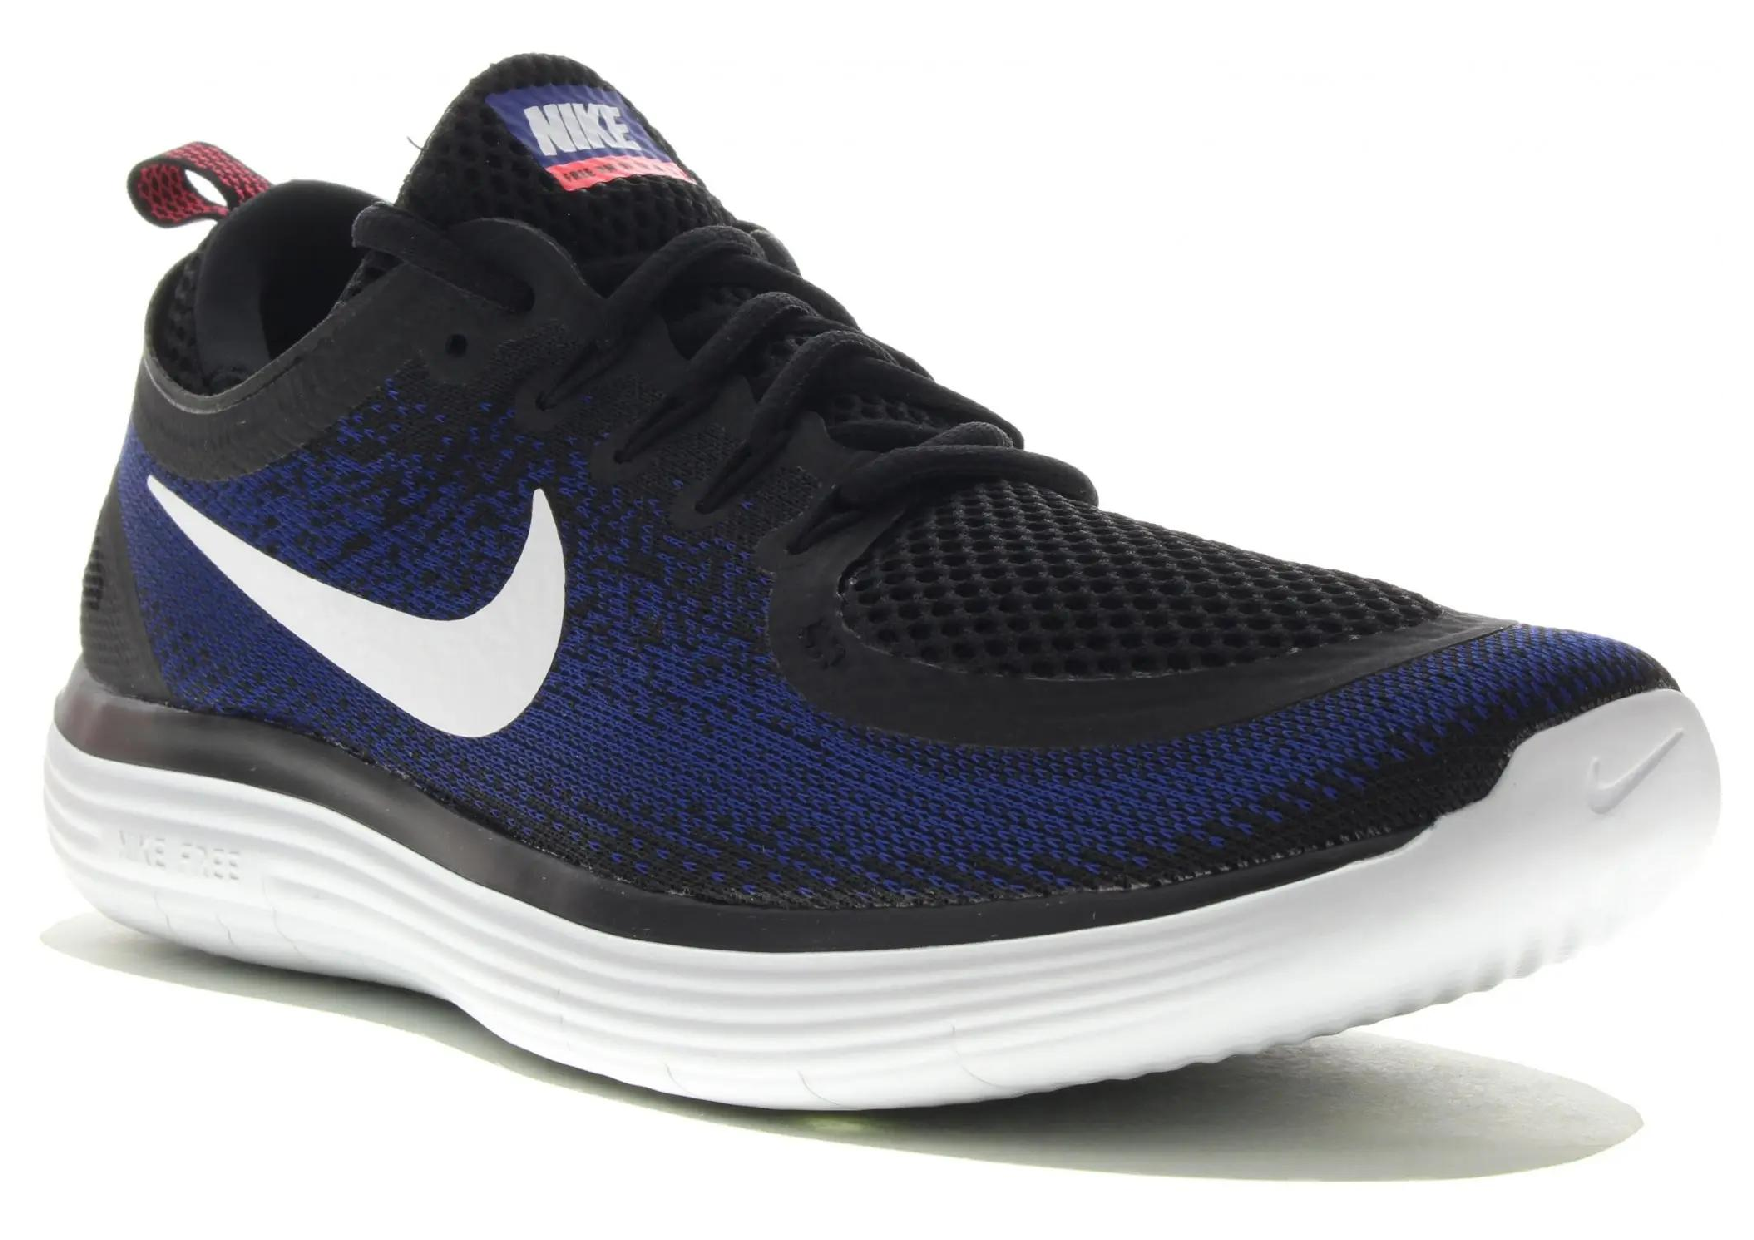
\includegraphics[scale=0.05]{fig/intro/motivation/lo_stakes/brand_new}};
            \node[align=center] at (img_brand_new.south) {The \emph{Nike Free RN Distance 2}};
        \end{tikzpicture}        
    \end{figure}
\end{frame}
 %--------------------------------------------------------------------------------------------------
\begin{frame}[t]
    \frametitle{Motivation: Raising the stakes}
    Now let's consider riskier situations:
    \pause
    \begin{figure}
        \centering
        \begin{tikzpicture}[font={\scriptsize}]
            \node (cancer) at (current page.north west) 
                {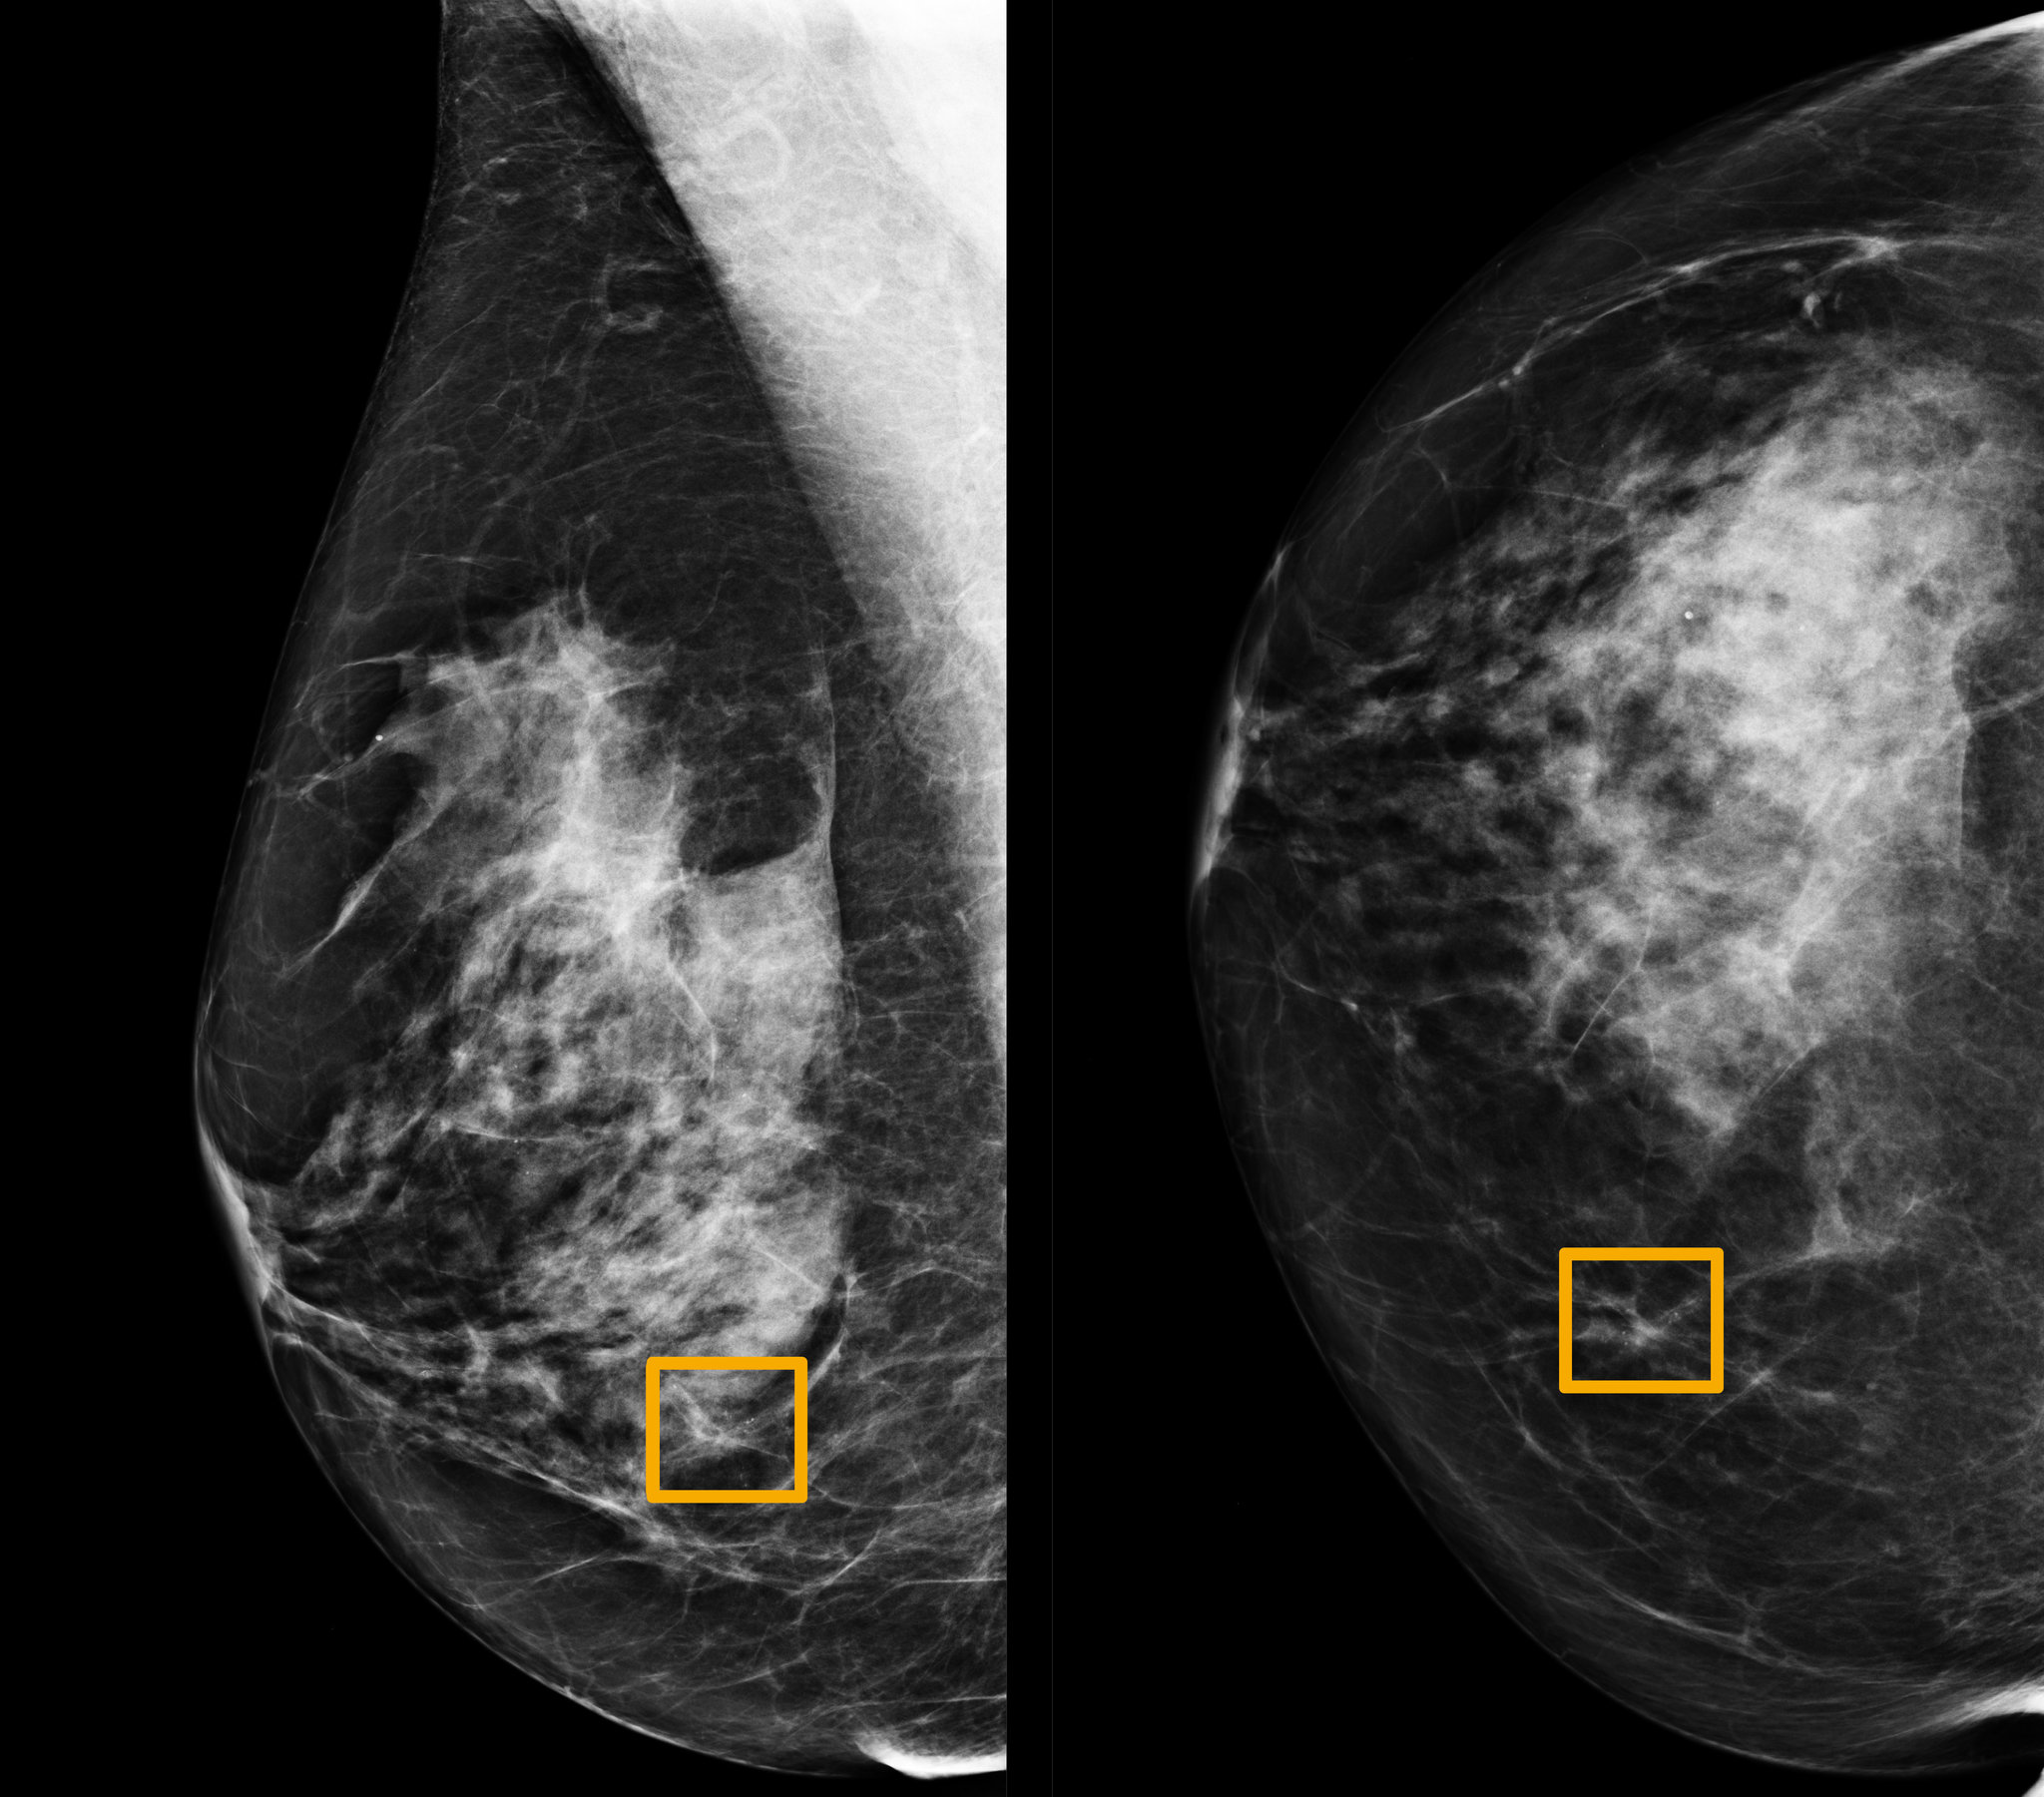
\includegraphics[scale=.07]{fig/intro/motivation/hi_stakes/breast_xray.jpg}};
            \pause
            \node (reid) at (cancer.south) {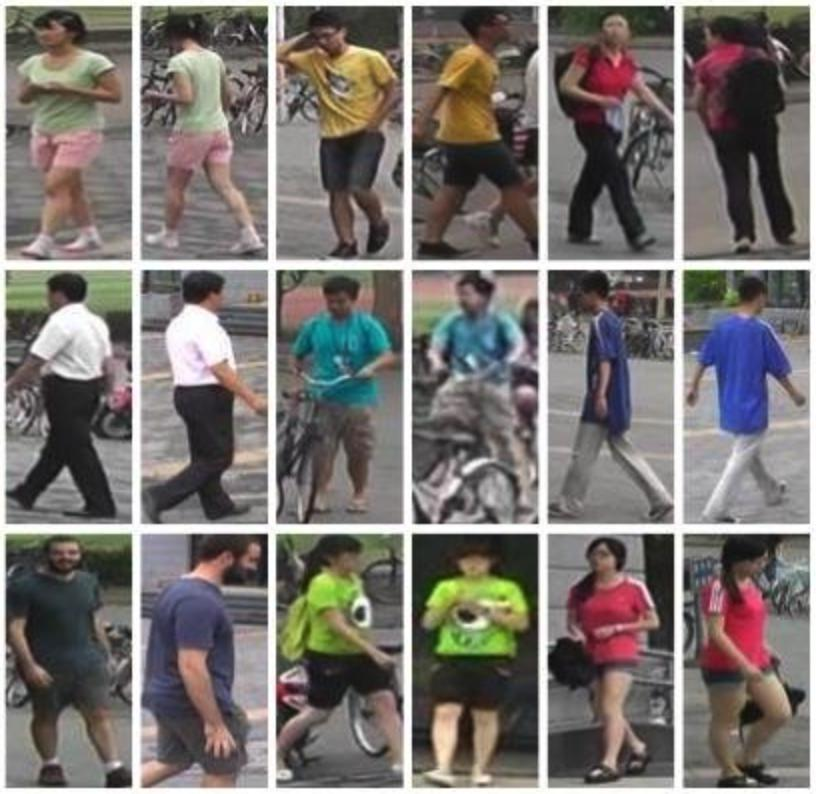
\includegraphics[scale=0.1]
                {fig/intro/motivation/hi_stakes/Market-1501.jpg}};
            \pause
            \node (roadkill) at (cancer.east) {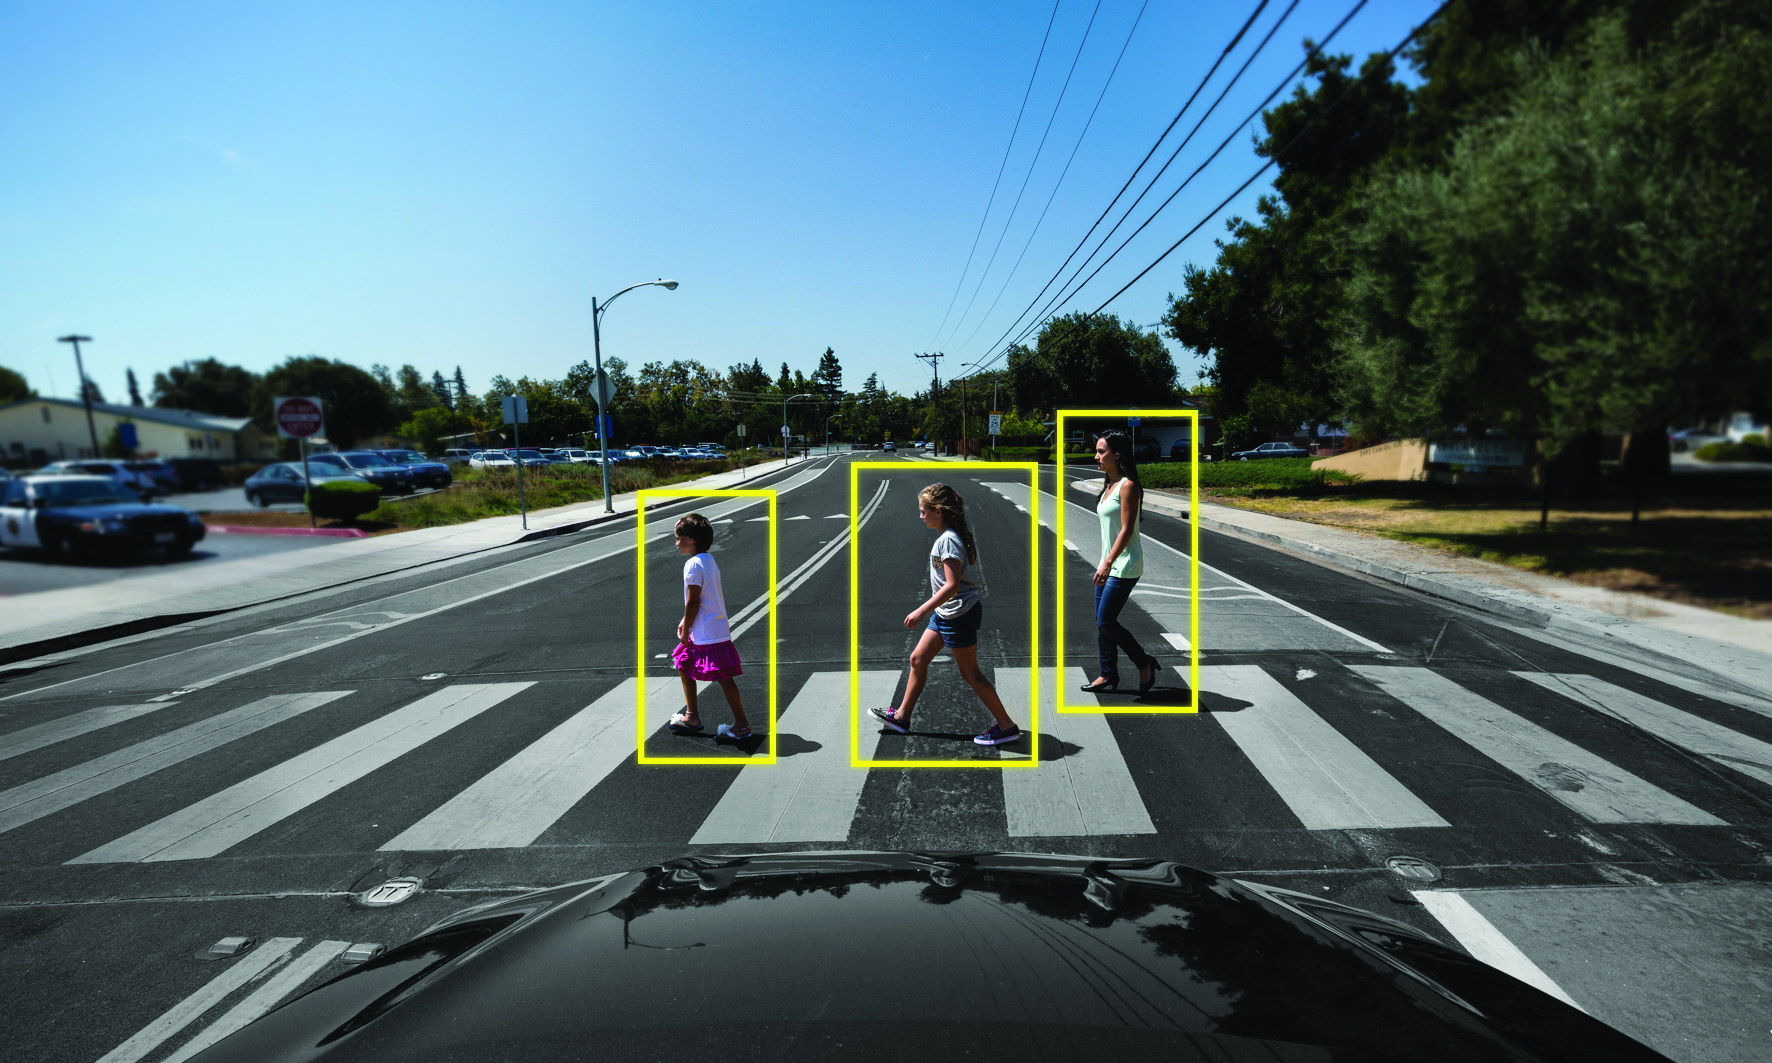
\includegraphics[scale=0.4]
                {fig/intro/motivation/hi_stakes/zebra_crossing.jpg}};
            
        \end{tikzpicture}
    \end{figure}
\end{frame}
 %--------------------------------------------------------------------------------------------------
 \begin{frame}[t]
    \frametitle{Motivation: Straight to the point}
    \begin{columns}
        \column{0.5\textwidth}
        \begin{figure}
            \centering
            \begin{tikzpicture}[font={\scriptsize}]
                \node (cancer) at (current page.north west) 
                    {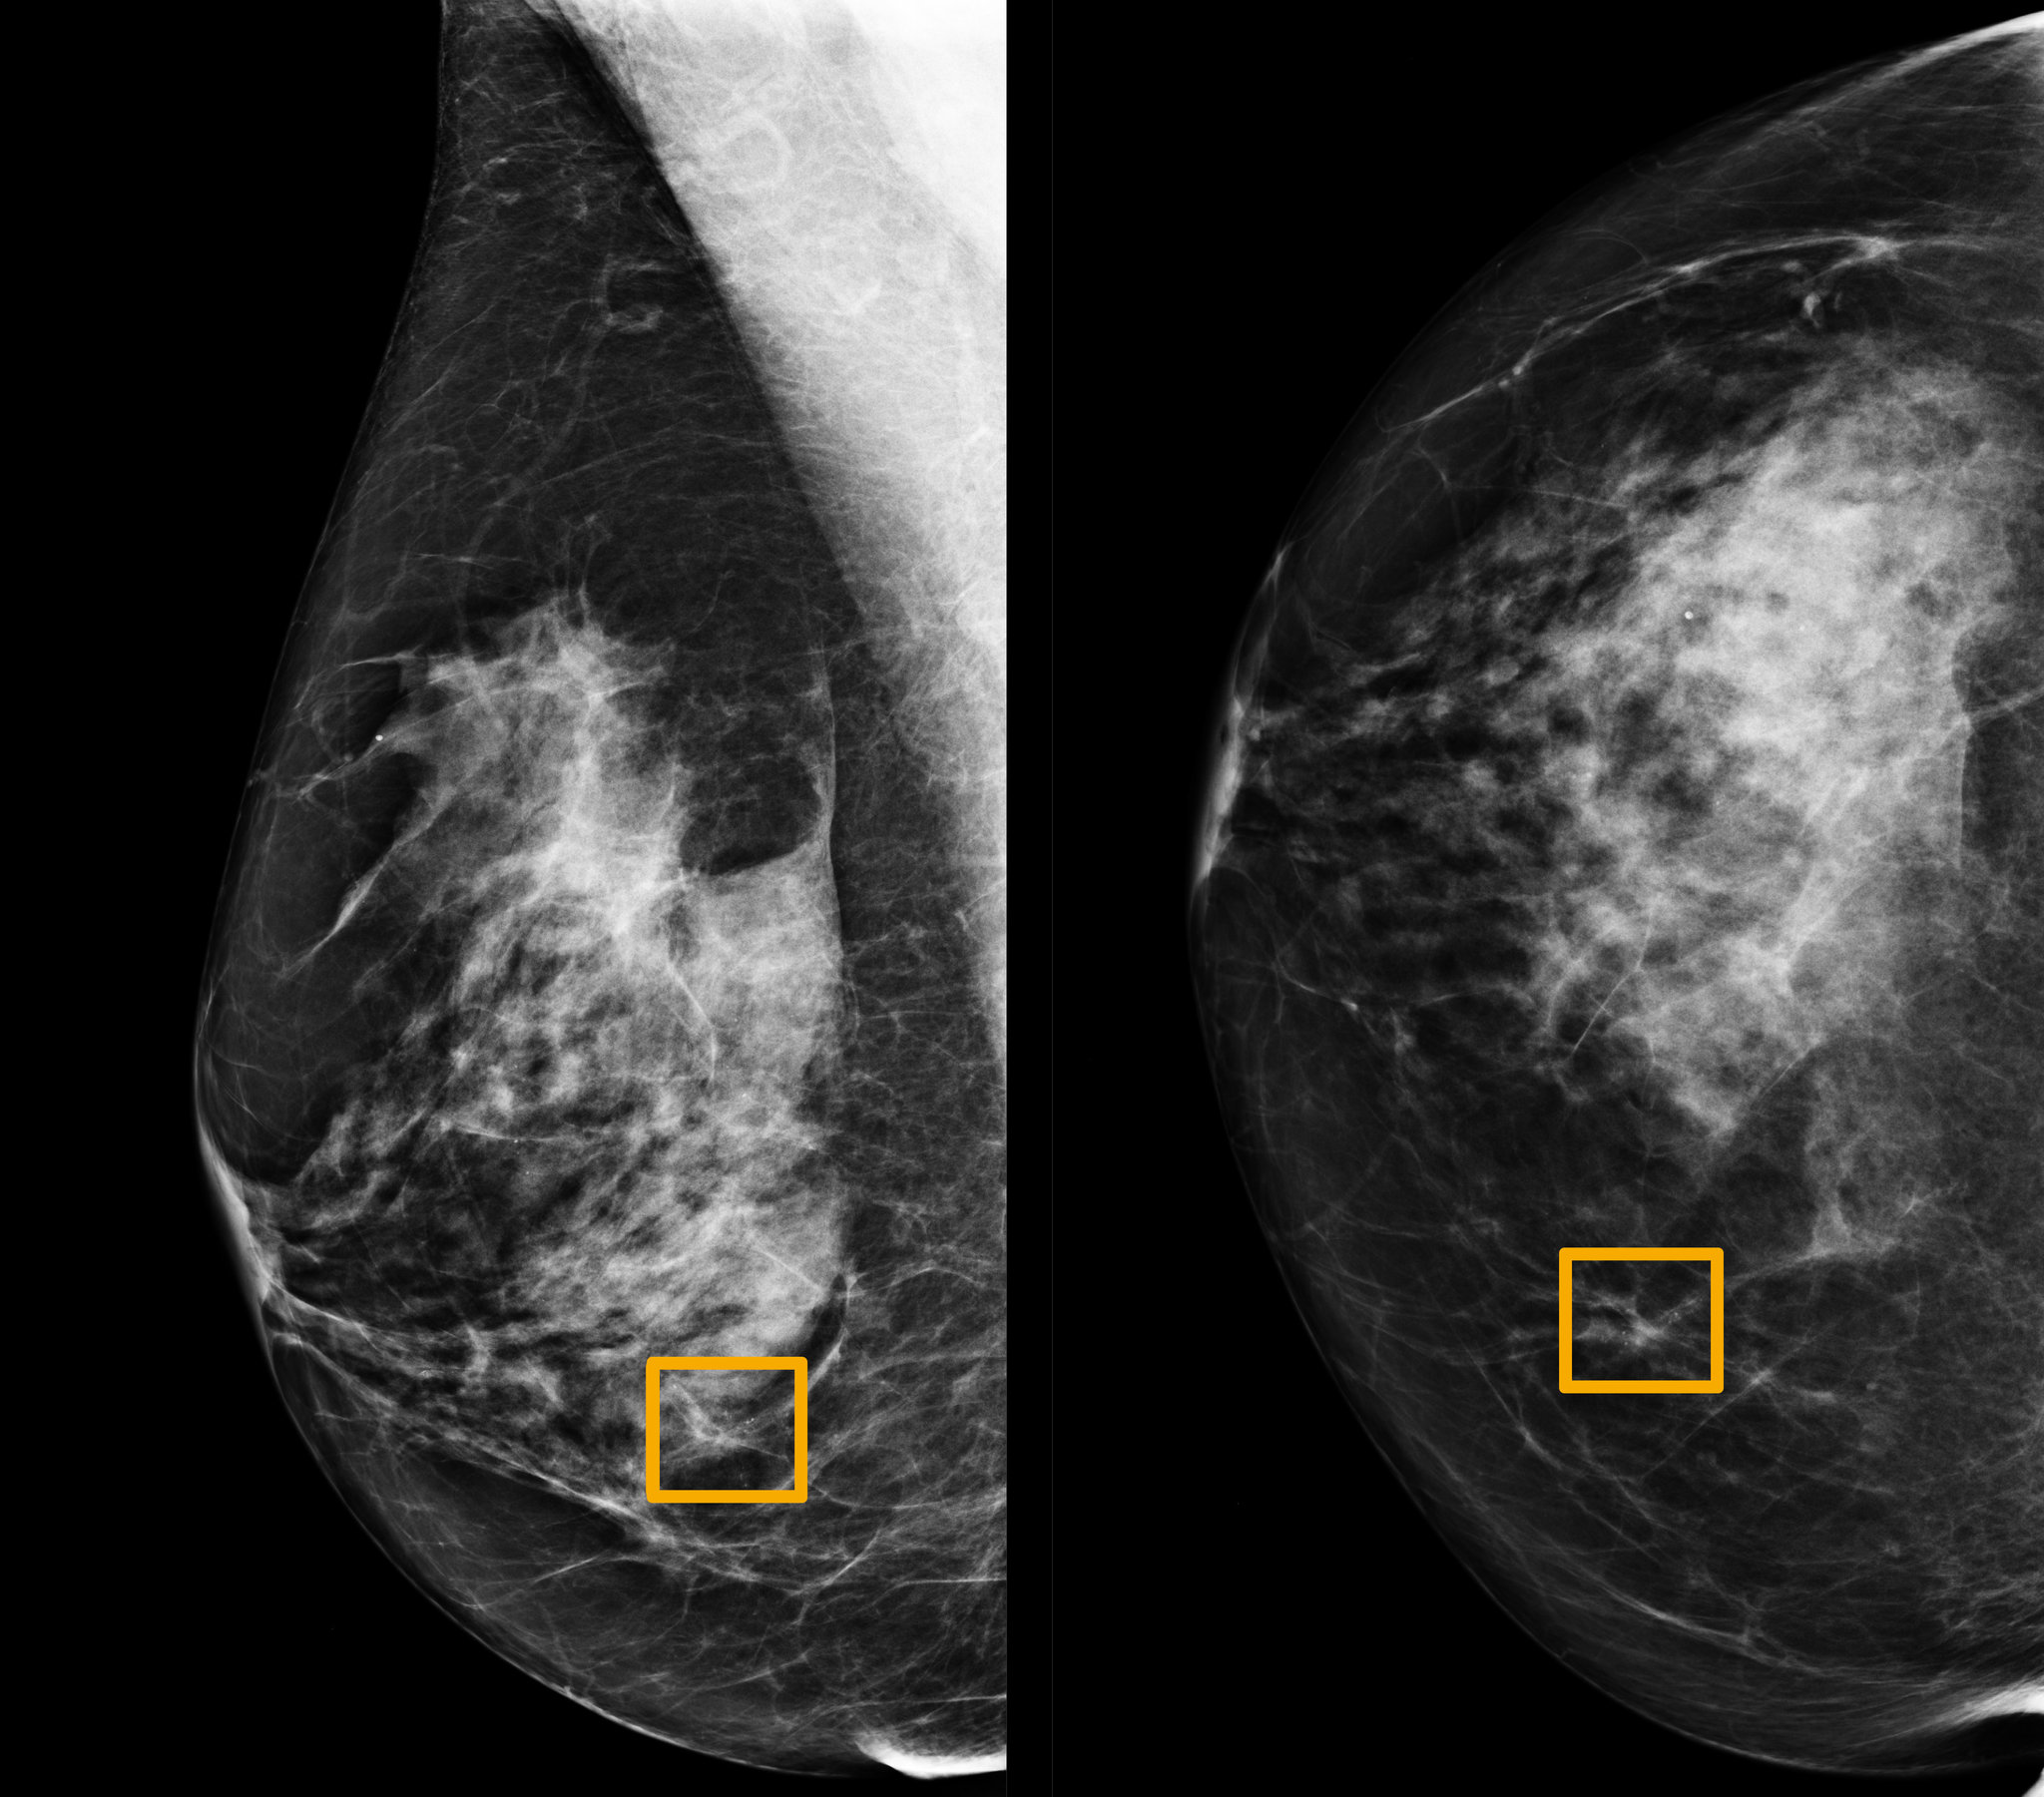
\includegraphics[scale=.05]{fig/intro/motivation/hi_stakes/breast_xray.jpg}};
                \node (roadkill) at (cancer.south) 
                    {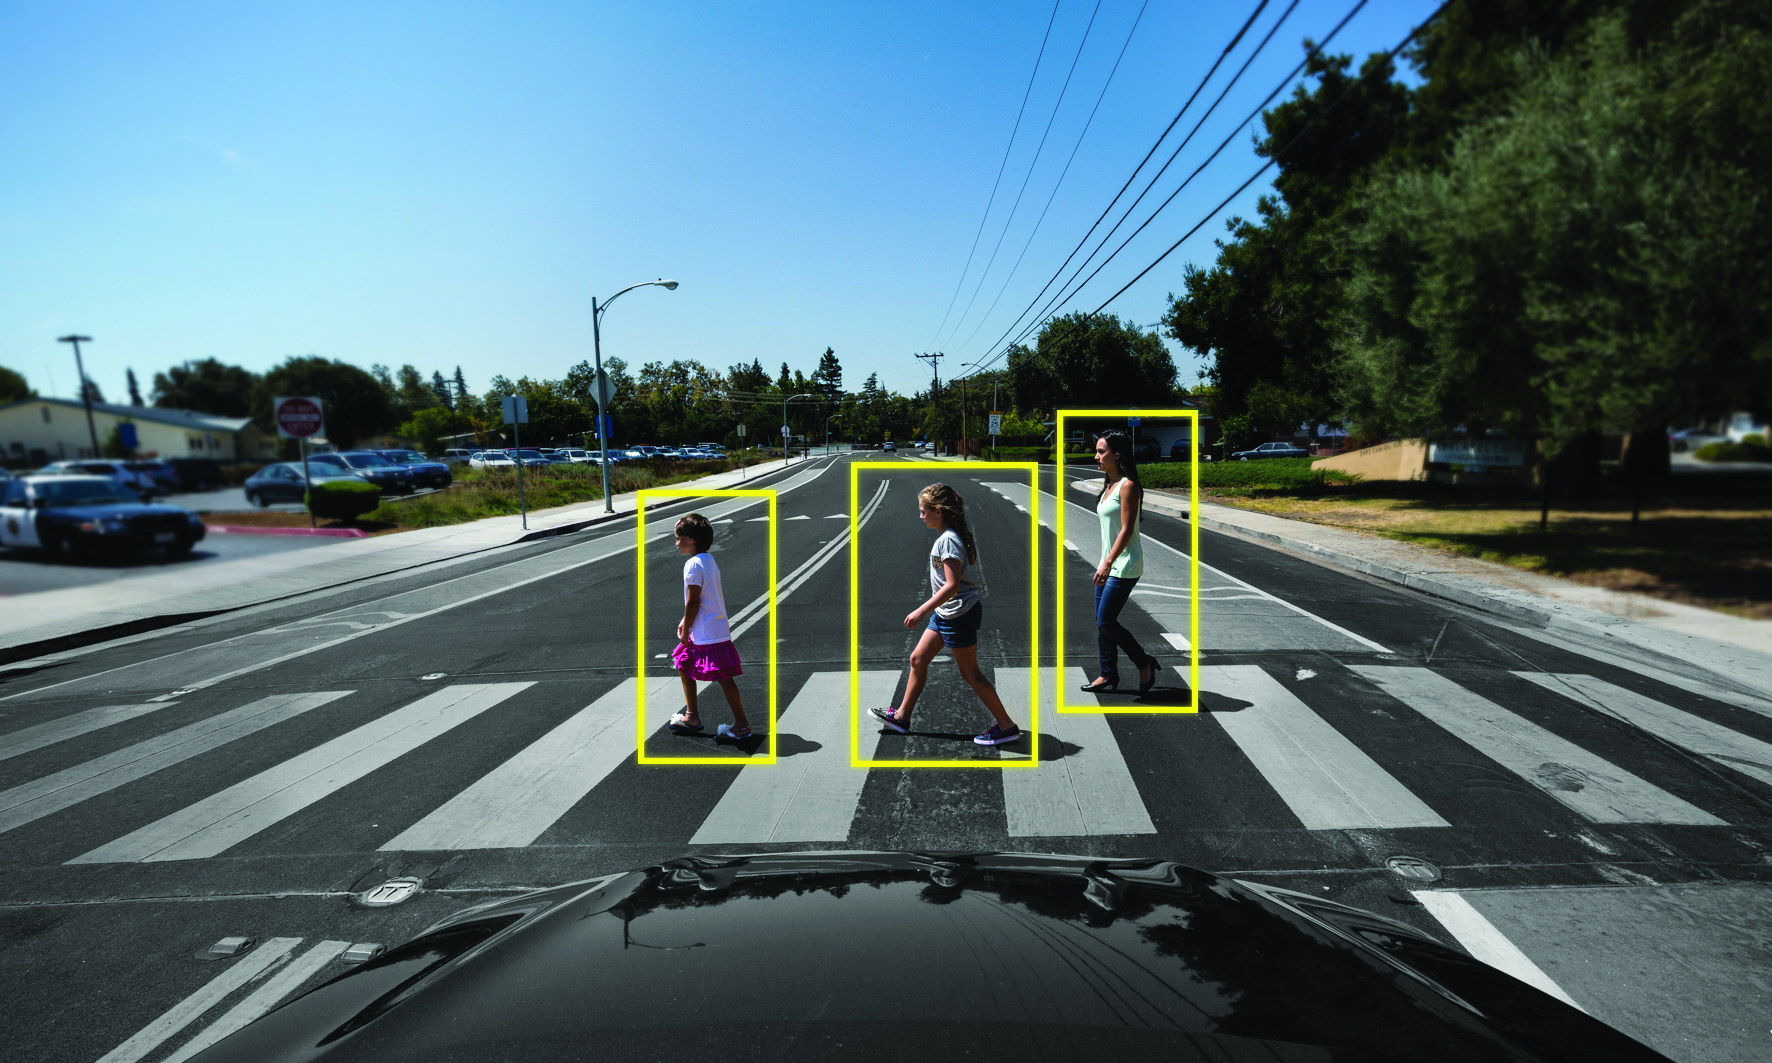
\includegraphics[scale=0.282]{fig/intro/motivation/hi_stakes/zebra_crossing.jpg}};
                \node (reid) at (roadkill.north east) 
                    {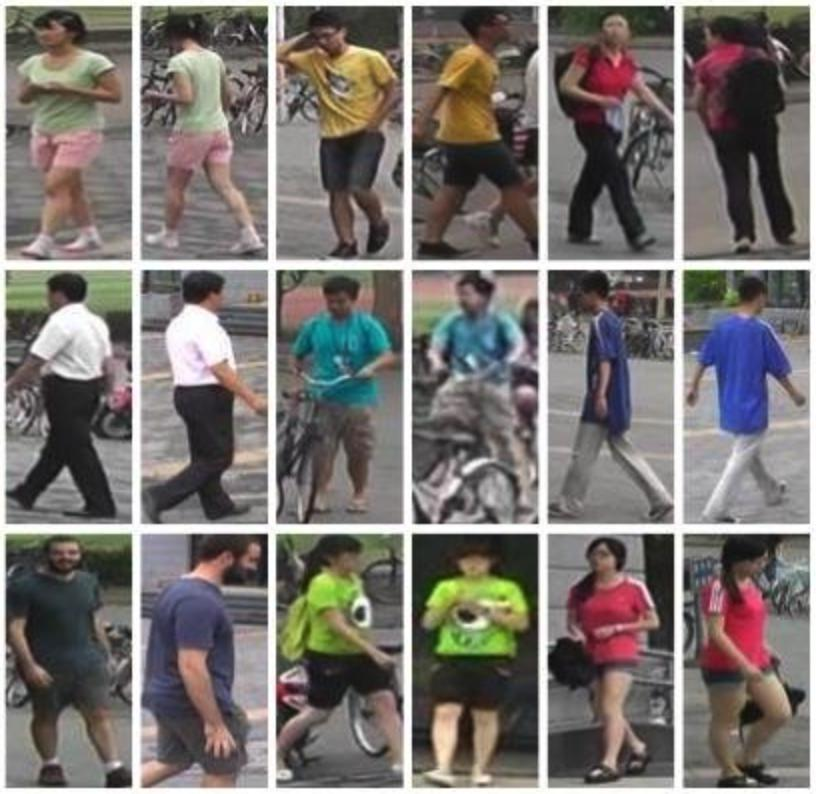
\includegraphics[scale=0.0883]{fig/intro/motivation/hi_stakes/Market-1501.jpg}};                
            \end{tikzpicture}
        \end{figure}
        \column{0.5\textwidth}
            \begin{itemize}
                \item How do we know \textbf{how} safe a system is?\pause
                \item How do we \textbf{know} how a system works?\pause
                \item If a system fails, \textbf{who} is accountable?
            \end{itemize}
        \end{columns}
 \end{frame}
 %--------------------------------------------------------------------------------------------------
\begin{frame}
    \frametitle{}
    \centering
    Let's slow for a bit\\
    and go step by step:   
\end{frame}
%--------------------------------------------------------------------------------------------------
\subsection*{Computation, Computer Vision and AI}
\begin{frame}[t]
    \frametitle{Computation, Computer Vision and AI}
    \cite{mythos_interp}
\end{frame}
\subsection*{Objectives}
%--------------------------------------------------------------------------------------------------
\begin{frame}[t]
    \frametitle{Thesis Objectives}
    \textbf{Improvement of recognition and interpratable properties of model predictions.}\\
    \vspace{20pt}
    \pause    
    In particular:
    \begin{itemize}
        \item Development of low cost/complexity explainability approaches.
        \item Establishment of a fixed evaluation protocol. 
        \item Differenciation of human based and machine explanations.
    \end{itemize}

\end{frame}

	\section{Background}
%--------------------------------------------------------------------------------------------------
\begin{frame}[t]
    \frametitle{Background}
    To familiarize with this work, we split it into three points:\\\pause
    \begin{columns}[t]
        \column{.275\textwidth}
        \begin{center}
            \footnotesize\textbf{Preliminaries}\\
            \begin{itemize}
                \footnotesize\item Approaching Vision.
                \footnotesize\item David Marr's approach.
                \footnotesize\item CV currently.
                \footnotesize\item Desiredata of Interpretability Study.
            \end{itemize}
        \end{center}
        \column{.375\textwidth}
        \begin{center}
            \footnotesize\textbf{Image Recognition Models}\\
            \begin{itemize}
                \footnotesize\item Traditional Models.
                \footnotesize\item Convolutional Neural Networks (CNN).
                \footnotesize\item Hybrid Architectures.
            \end{itemize}
        \end{center}
        \column{.4\textwidth}
        \begin{center}
            \footnotesize\textbf{Interpretability}\\
            \begin{itemize}
                \footnotesize\item Transparency.
                \footnotesize\item Post-Hoc Interpretability.
                \begin{itemize}
                    \footnotesize\item Class Activation Methods.
                \end{itemize}
                \footnotesize\item Evaluating Interpretability.
            \end{itemize}
        \end{center}
    \end{columns}            
\end{frame}
\subsection*{Preliminaries}
%--------------------------------------------------------------------------------------------------
\begin{frame}[t]
    \frametitle{Preliminaries}
    \framesubtitle{Approaching Vision}
    
\end{frame}
%--------------------------------------------------------------------------------------------------
\begin{frame}[t]
    \frametitle{Preliminaries}
    \framesubtitle{David Marr's approach}
    \begin{columns}[t]
        \column{0.5\textwidth}
        \begin{center}
            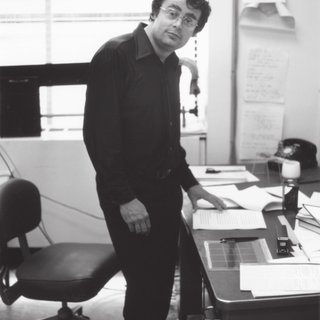
\includegraphics[width=0.8\textwidth]{fig/rel/common/img/Marr.jpg}    
        \end{center}
        \column{0.5\textwidth}
        Addressing vision on three levels:
        \begin{itemize}
            \item Algorithmic.
            \item Implementation.
            \item Computational.
            \begin{itemize}
                \item Three fundamental tasks. \cite{malik2016three}
            \end{itemize}
        \end{itemize}
        \pause
        \vspace{20pt}
        \textbf{Computer Vision focuses on the last level.}
        
    \end{columns}
    
\end{frame}
%--------------------------------------------------------------------------------------------------
\begin{frame}[t]
    \frametitle{Preliminaries}
    \framesubtitle{CV Currently}
    
    
\end{frame}
%--------------------------------------------------------------------------------------------------
\begin{frame}[t]
    \frametitle{Preliminaries}
    \framesubtitle{Desiredata of Interpretability Study}
    \begin{columns}[c]
        \column[T]{0.4\textwidth} 
        {\footnotesize%           
         We ask  questions regarding \emph{black box models}.
         \begin{itemize}
             \item How does it work?
             \item How safe is it?
             \item Who is accountable for it?
             \item Who benefits from it?
             \item Who uses it?.
         \end{itemize}
         \vspace{20pt}
         \textbf{Accepted AI systems within society must answer this.}
        }
        \column[T]{0.6\textwidth}
        \pause
        \begin{center}
            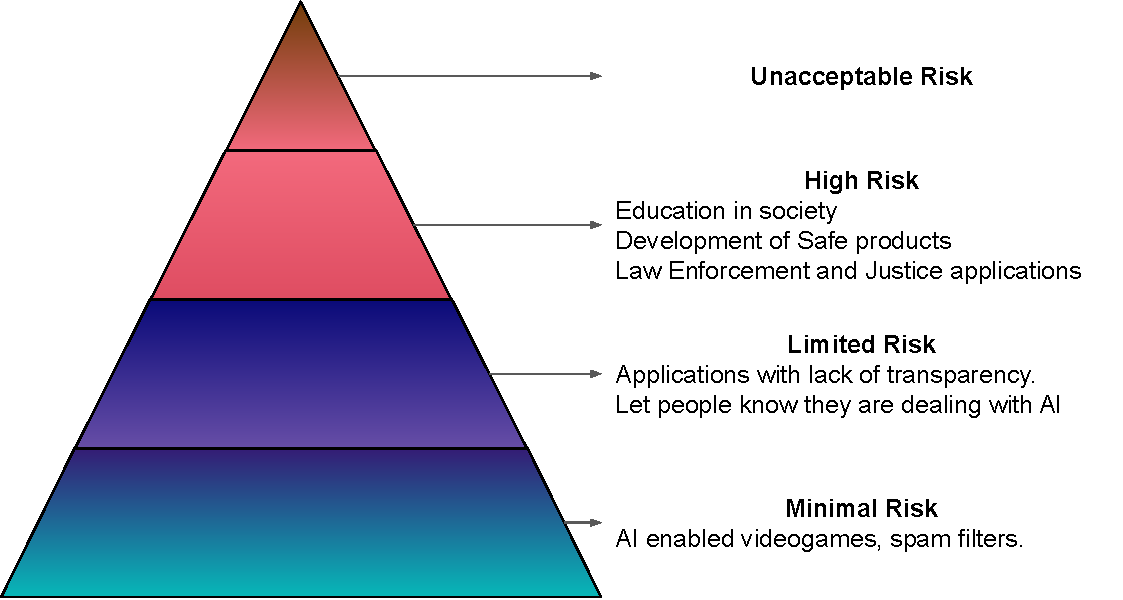
\includegraphics[width=\textwidth]{fig/rel/common/img/AI_act_pyramid.pdf}      
            \footnotesize Regulation planned with the European AI act\cite{madiega2021artificial}
        \end{center}

    \end{columns}
    
\end{frame}
\subsection*{Image Recognition Models}
%--------------------------------------------------------------------------------------------------
\begin{frame}[t]
    \frametitle{Image Recognition Models}
    \framesubtitle{Classic Models}
\end{frame}
%--------------------------------------------------------------------------------------------------
\begin{frame}[t]
    \frametitle{Image Recognition Models}
    \framesubtitle{Convolutional Neural Networks}
    \begin{columns}
        \column[T]{0.5\textwidth}
        {\footnotesize Based on the \textbf{convolution operation}.\\
         A representation $f\star g$ is computed for a feature map $f$ and a kernel $g$.\\
         First approach with \emph{Neocognitron} \cite{fukushima1975cognitron}}
        \column[T]{0.5\textwidth}
            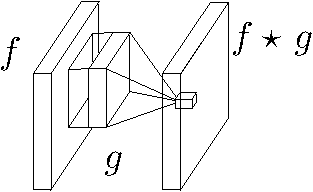
\includegraphics[scale=0.75]{fig/rel/imrecon/img/conv_schema.pdf}
    \end{columns}\pause
    \begin{center}
        {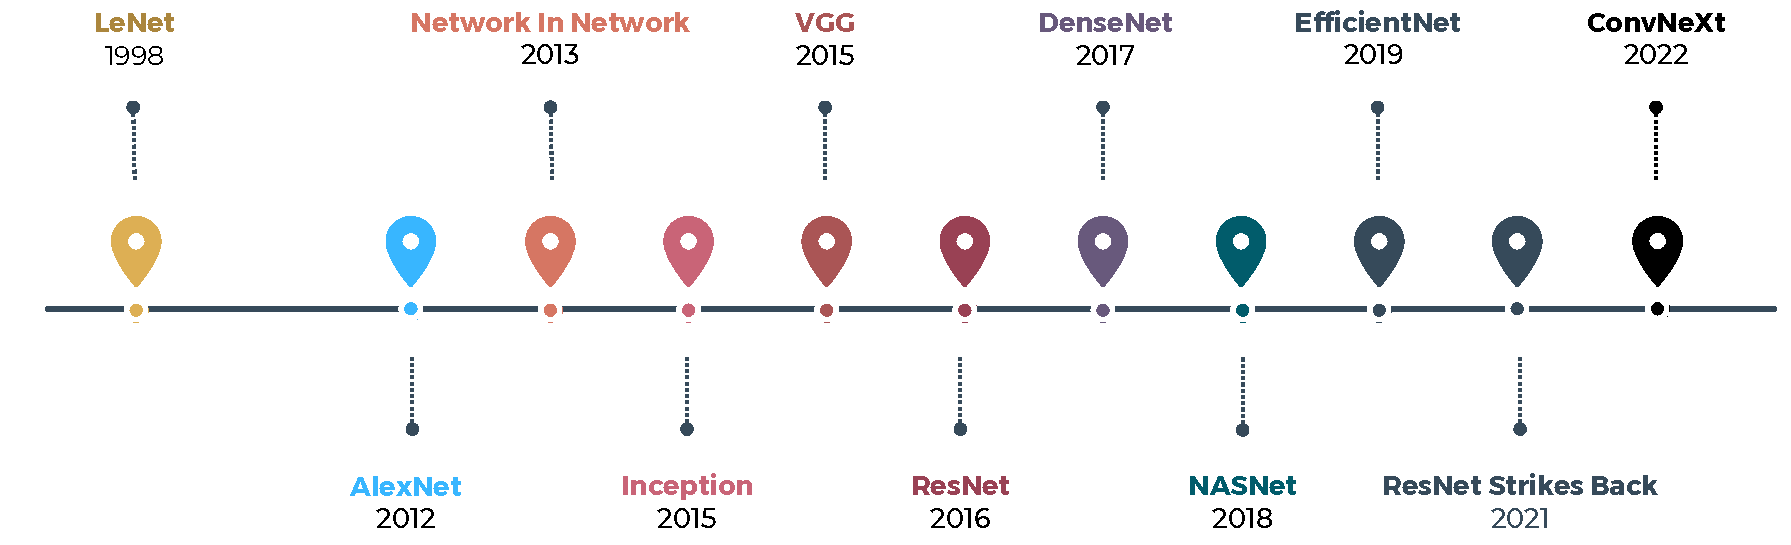
\includegraphics[width=\textwidth]{fig/rel/imrecon/img/CNN_timeline.pdf}}
    \end{center}
        
\end{frame}
%--------------------------------------------------------------------------------------------------
\begin{frame}[t]
    \frametitle{Image Recognition Models}
    \framesubtitle{Self Attention Architectures}
    \begin{columns}
        \column[T]{.5\textwidth}
         {\footnotesize Updates a representation, using the relevance of each element relative to others in an 
         embedding.\\
         An input is projected to three spaces ($Q K V$), the weights control the relevance of each 
         element.}
        \column[T]{.5\textwidth}
        \begin{center}
            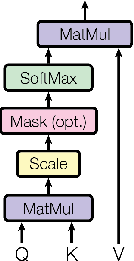
\includegraphics[width=0.5\textwidth]{fig/rel/imrecon/img/scaled_dotproduct.pdf}
        \end{center}
        
    \end{columns}
    
\end{frame}
%--------------------------------------------------------------------------------------------------
\begin{frame}[t]
    \frametitle{Image Recognition Models}
    \framesubtitle{The Current Landscape}
    Transformers had a strong impact on image recognition. 
    %--------------------------------------------------------------------------------------------------
\pgfplotstableread[col sep=comma,]{fig/rel/data/models_year.csv}\datatable
    \begin{tikzpicture}
        \begin{axis}[
            %font={\scriptsize},
            date coordinates in=x,
            date ZERO=2017-03-31,
            xtick distance=0.25,
            %xtick={\datatable}{Year},
            %xticklabel={\year-\month-\day},
            xtick=data,
            width=\textwidth,
            height=6.5cm,
            xticklabel style={rotate=90, anchor=near xticklabel},
            ylabel={Proportion of Papers (Quarterly)},
            legend style={at={(0, 1)}, anchor=north west},
            yticklabel style={/pgf/number format/fixed}
            ]
            \tikzstyle{every node}=[font=\scriptsize]
            \addplot [mark=*, red!80] table [x={Year}, y={ResNet}]{\datatable};
            \addlegendentry{{\tiny \Th{ResNet}}}

            \addplot [mark=*, black!80] table [x={Year}, y={VGG}]{\datatable};
            \addlegendentry{{\tiny \Th{VGG}}}

            \addplot [mark=*, green!80] table [x={Year}, y={DenseNet}]{\datatable};
            \addlegendentry{{\tiny\Th{DenseNet}}}

            \addplot [mark=*, cyan!80] table [x={Year}, y={EfficientNet}]{\datatable};
            \addlegendentry{{\tiny \Th{EfficientNet}}}

            \addplot [mark=*, blue!80] table [x={Year}, y={ViT}]{\datatable};
            \addlegendentry{{\tiny \Th{ViT}}}
        \end{axis}
    \end{tikzpicture}
%    \caption{\textbf{Proportion of articles published on ImageNet,} using image recognition models as backbone across the years. 
%             Original from \url{https://paperswithcode.com/method/resnet}}
%    \label{fig:paradigmn_shift}
%\end{figure}
    
\end{frame}
\subsection*{Interpretability}
%--------------------------------------------------------------------------------------------------
\begin{frame}[t]
    \frametitle{Interpretability}
    \framesubtitle{Transparency}
\end{frame}
%--------------------------------------------------------------------------------------------------
\begin{frame}[t]
    \frametitle{Interpretability}
    \framesubtitle{Post-Hoc Interpretability}
    
\end{frame}
%--------------------------------------------------------------------------------------------------
\begin{frame}[t]
    \frametitle{Interpretability}
    \framesubtitle{Class Activation Methods}
\end{frame}
%--------------------------------------------------------------------------------------------------
\begin{frame}[t]
    \frametitle{Interpretability}
    \framesubtitle{Evaluating Interpretability}
\end{frame}
	\section[Opti-CAM]{Opti-CAM: Optimizing saliency maps for interpretability}

	\section[CA-Stream]{CA-Stream: Attention-based pooling for interpretable image recognition}
\begin{frame}
    %\cite{petsiuk2018rise}
\end{frame}
	\section[Gradient]{A learning paradigm for interpretable gradients}

	\nonumsec{References}
%\addcontentsline{toc}{section*}{References}
%--------------------------------------------------------------------------------------------------
\begin{frame}[allowframebreaks]
    \frametitle{References}
    \bibliographystyle{IEEEtran}
    \bibliography{biblio}
\end{frame}


	%-----------------------------------------------------------------------------------------------
\end{document}